\documentclass[main]{subfiles}

\begin{document}

\chapter{Ingenier\'ia inversa}

El cuadric\'optero adquirido resuelve la comunicaci\'on entre los controladores de los motores (\textbf{ESCs}) y el microprocesador mediante el protocolo $\mathbf{i^2c}$.\\

Para el presente proyecto resulta de vital importancia conocer dicho protocolo, ya que se utilizar\'a otro microprocesador que deber\'a comandar a esos mismos ESCs, supliendo el trabajo del anterior. Es entonces imprescindible conocer al detalle el funcionamiento de este protocolo, para luego poder reproducirlo.\\

Dado que no se cuenta con la mínima colaboraci\'on de los fabricantes y la informaci\'on es completamente privativa, es necesario realizar un proceso de ingenier\'ia inversa para poder analizar, decodificar, entender y reproducir el protocolo existente. Dicho proceso de ingenier\'ia inversa se realiza utilizando el hardware existente del cuadric\'optero comercial adquirido y un analizador l\'ogico\footnote{ChronoVu} que es capaz de leer e interpretar las l\'ineas del bus $i^2c$ sin intervenir en las mismas.\\ \\

\begin{wrapfigure}{r}{0.5\textwidth}
	\vspace{-40pt}
	\begin{center}
	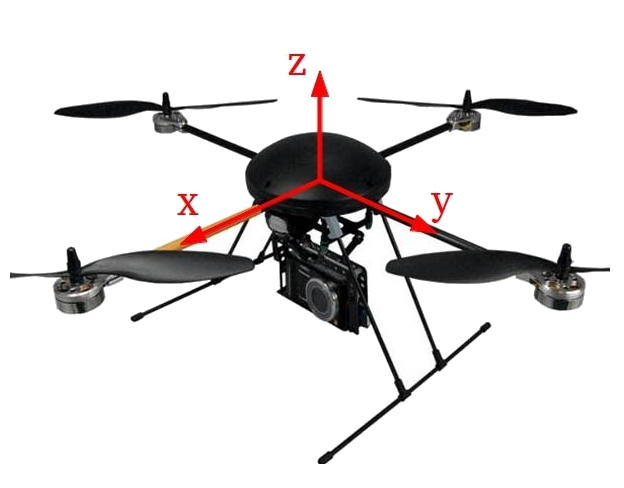
\includegraphics[width=0.4\textwidth]{./pics_sniffer/ejes_quad.jpg}
	\end{center}
	\vspace{-20pt}
	\caption{Definici\'on de ejes}
	\label{fig:ejes_quad}
	\vspace{-70pt}
\end{wrapfigure}

Antes de presentar los resultados obtenidos en el proceso, se realiza una breve introducci\'on al protocolo $i^2c$. En la figura \ref{fig:ejes_quad} se presenta la definici\'on de los ejes a utilizar, lo cual ser\'a de utilidad m\'as adelante.

\newpage
\section{Introducci\'on al protocolo $i^2c$}

El bus $i^2c$ es un bus de comunicaciones serie. Su nombre viene de \emph{Inter-Integrated Circuit} (Circuitos Inter-Integrados).\\
Utiliza dos l\'ineas para transmitir la informaci\'on: una para los datos y otra para la señal de reloj. Adem\'as ser\'a necesaria una tercera l\'inea de tierra, como referencia.\\
En la imagen \ref{fig:setup}\footnote{Imagen tomada de www.i2c-bus.org} se muestra un diagrama de un circuito equivalente simplificado de la conexi\'on $i^2c$ entre 2 dispositivos.

\begin{figure}[h!]
	\centering
	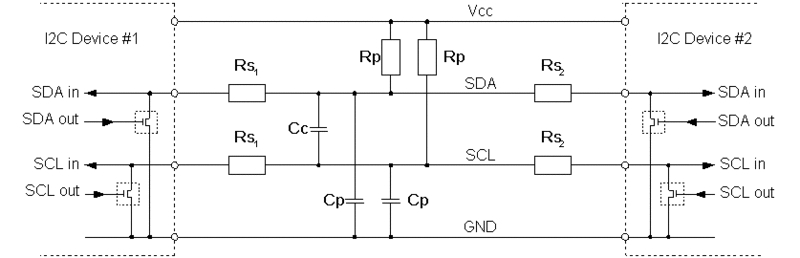
\includegraphics[width=0.8\textwidth]{./pics_sniffer/setup.jpg}
	\caption{Conexi\'on $i^2c$.}
	\label{fig:setup}
\end{figure}
donde:
\begin{itemize}
\item \verb+Vcc+:	 Voltaje de entrada, t\'ipicamente var\'ia entre 1.2 V y 5.5 V
\item \verb+GND+:	 Tierra com\'un
\item \verb+SDA+:	 L\'inea serial de datos
\item \verb+SCL+:	 L\'inea serial de reloj
\item \verb+Rp+ :	 Resistencia de "Pull-up"
\item \verb+Rs+ :	 Resistencia serie
\item \verb+Cp+ :	 Capacitancia del cable
\item \verb+Cc+ :	 Capacitancia de canal cruzado
\end{itemize}

Las l\'ineas \textbf{SDA} y \textbf{SCL} son de drenador abierto, lo que significa que tanto el maestro como los esclavos solamente pueden conducir a nivel bajo estas l\'ineas, o dejarlas abiertas. Si ning\'un dispositivo $i^2c$ est\'a conduciendo hacia abajo la l\'inea, la resistencia de \emph{pull-up} $R_p$ se encarga de llevar la l\'inea a $V_{cc}$.\\

El reloj siempre es generado por el maestro. El bus de datos debe mantenerse estable mientras el reloj está en nivel alto (``1'' lógico) y se le permite cambiar de nivel mientras el reloj está en nivel bajo (``0'' lógico). Se toma como dato válido el valor del bus de datos cuando el reloj está en ``0''.\\

Cada dispositivo tiene asignada una direcci\'on que lo identifica. Típicamente para establecer una comunicaci\'on el maestro env\'ia una secuencia de comienzo de conexi\'on, seguida de la direcci\'on del esclavo con el cual desea comunicarse. Seguidamente el maestro env\'ia un bit que determina si la acci\'on que desea realizar es escritura o lectura, a lo que el esclavo correspondiente responde con un bit de \emph{acknowledge} (\textbf{Ack}). Luego el maestro env\'ia la direcci\'on de memoria interna del esclavo donde debe ser almacenada la informaci\'on enviada, y por \'ultimo env\'ia los datos. Para finalizar la conexi\'on, el maestro env\'ia una secuencia de fin de conexi\'on.

\section{Pruebas en r\'egimen}

\begin{itemize}
	\item Materiales
	\begin{itemize}
		\item \emph{Cuadricóptero:} transmisor, receptor, CPU y ESCs
		\item \emph{Analizador lógico (``sniffer''):} Chrono Vu
		\item \emph{PC}
	\end{itemize}
	\item Procedimiento
	\begin{itemize}
		\item La forma de operar es enviar comandos conocidos con el control remoto y analizar el flujo de datos en las l\'ineas del bus.
		\item En particular se analizará el funcionamiento en régimen, durante el arranque y durante el frenado.
	\end{itemize}
\end{itemize}

La comunicación entre la CPU y los ESCs es mediante el protocolo $i^2c$, y es precisamente allí donde interviene el analizador lógico, ``olfateando'' todo lo que pasa por el bus. En la figura \ref{fig:sniffing_diagram} se muestra un diagrama de bloques del proceso descripto, y en la figura \ref{fig:sniffing_transparente} su implementación.

\begin{figure} [h!]
\centering
  \subfloat[Diagrama de interconexión]{\label{fig:sniffing_diagram}
  		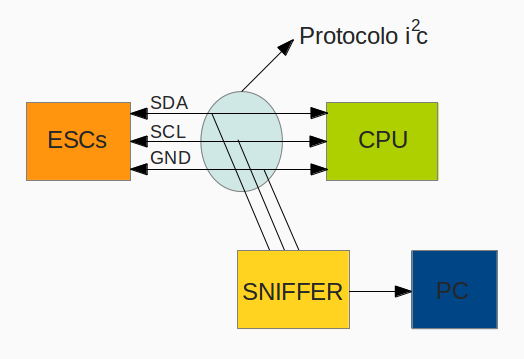
\includegraphics[width=.5\textwidth]{./pics_sniffer/sniffing_diagram.png}}
  \subfloat[Proceso de ``sniffeado'']{\label{fig:sniffing_transparente} 
  		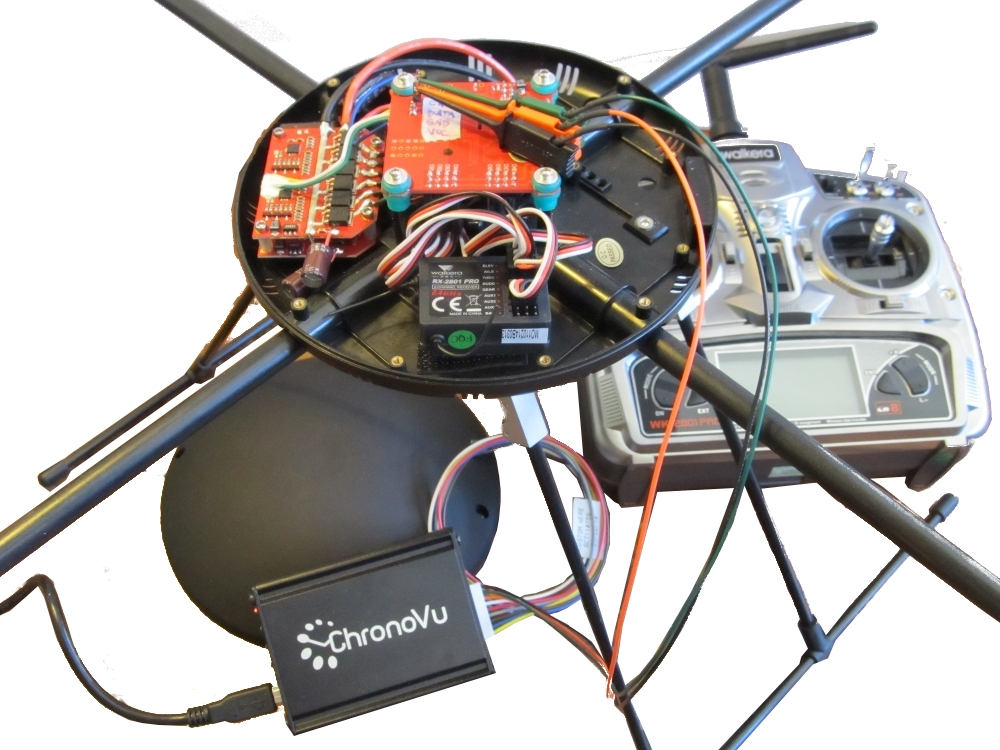
\includegraphics[width=.42\textwidth]{./pics_sniffer/sniffing_transparente.jpg}}
  \caption{Proceso de lectura del bus.}
  \label{fig:sniffing}
\end{figure}

Al realizar este proceso se puede observar que se repiten, cada $2ms$, bloques similares al mostrado en la figura \ref{fig:bloque_snif}.

\begin{figure}[h!]
	\centering
	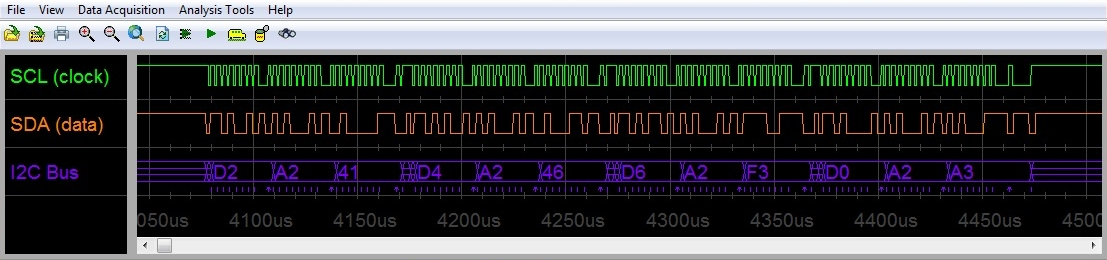
\includegraphics[width=1\textwidth]{./pics_sniffer/bloque_snif.jpg}
	\caption{Bloque de transmisi\'on $i^2c$}
	\label{fig:bloque_snif}
\end{figure}

De acuerdo a la observaci\'on de dichos bloques, teniendo en cuenta la secuencia de comunicación típica entre maestro y esclavos mencionada anteriormente, se deduce que hay 4 esclavos correspondientes a los 4 ESC's de los 4 motores, cuyas direcciones en hexadecimal son \textbf{D0}, \textbf{D2}, \textbf{D4} y \textbf{D6}. La direcci\'on de la memoria interna de los esclavos donde se almacenan los datos que env\'ia el maestro es, en todos los casos \textbf{A2}. Adem\'as el maestro env\'ia un tercer conjunto de datos que refiere, de alguna manera, a la velocidad con la que debe girar cada motor.
Este conjunto de \'ordenes, agrupadas por bloques como el que se muestra en la figura \ref{fig:bloque_snif}, se repite peri\'odicamente, indicando la velocidad con la que debe girar cada motor.\\

Para comprender las pruebas realizadas es importante dejar en claro algunos aspectos previos. En la figura \ref{fig:tx} se muestra el transmisor utilizado para enviar comandos al cuadric\'optero, un \textbf{Walkera WK-2801} y se indican los nombres de los mandos m\'as importantes del mismo.


\begin{wrapfigure}{l}{0.55\textwidth}
	\vspace{-20pt}
	\begin{center}
	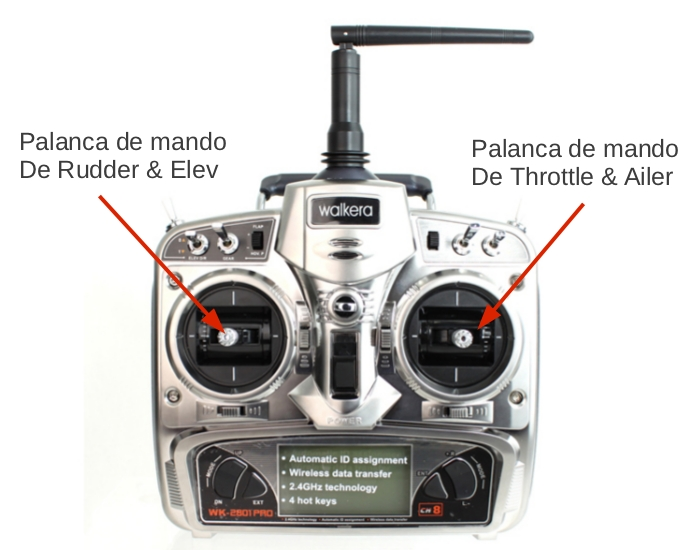
\includegraphics[width=0.45\textwidth]{./pics_sniffer/tx.jpg}
	\end{center}
	\vspace{-25pt}
	\caption{Transmisor}
	\label{fig:tx}
	\vspace{20pt}
\end{wrapfigure}

Al mover el mando de la izquierda (\textbf{Elev/Rudder}) en la direcci\'on vertical (\textbf{Elev}) se logra que el cuadric\'optero se eleve verticalmente, dando igual potencia a todos los motores, mientras que al moverlo en la direcci\'on horizontal, el cuadric\'optero presenta un movimiento de rotaci\'on seg\'un su eje vertical.\\

Al mover el mando de la derecha (\textbf{Throttle/Aile}) en la direcci\'on horizontal (\textbf{Aile}) y vertical (\textbf{Throttle}), se logran movimientos de rotaci\'on seg\'un los ejes horizontales \emph{x} e \emph{y} del cuadric\'optero. Las definiciones de los ejes se pueden ver en la figura \ref{fig:ejes_quad}.\\

Se analizan las siguientes situaciones:
\begin{table}[H]
\begin{center}
\begin{tabular}{|p{30pt}|c|c|c|c|p{130pt}|} 
\hline \cellcolor[gray]{0.8} \centering \textbf{Id} & \cellcolor[gray]{0.8} \textbf{Elev} & \cellcolor[gray]{0.8} \textbf{Ruddle} & \cellcolor[gray]{0.8} \textbf{Aile} & \cellcolor[gray]{0.8} \textbf{Throttle} & \cellcolor[gray]{0.8} \textbf{Movimiento}  \\ \hline
\centering 0 & atr\'as& medio & medio & medio & idle \\ \hline
\centering 1 & medio & medio & medio & medio & vertical hacia arriba con aceleraci\'on constante \\ \hline
\centering 2 & adelante & medio & medio & medio & vertical hacia arriba con aceleraci\'on constante \\ \hline
\centering 3 & medio & izquierda & medio & medio & giro seg\'un eje $z$ \\ \hline
\centering 4 & medio & derecha & medio & medio &  giro seg\'un eje $-z$ \\ \hline
\centering 5 & medio & medio & izquierda & medio & giro seg\'un eje $-x$  \\ \hline
\centering 6 & medio & medio & derecha & medio & giro seg\'un eje $x$  \\ \hline
\centering 7 & medio & medio & medio & atr\'as & giro seg\'un eje $-y$  \\ \hline
\centering 8 & medio & medio & medio & adelante & giro seg\'un eje $y$  \\ \hline
\end{tabular} 
\end{center}
\caption{Pruebas realizadas}
\label{tab:pruebas}
\end{table}

Se realiza un an\'alisis de los resultados obtenidos para cada motor, graficando el contenido del byte de datos que se le transmite a cada motor. Se obtienen representaciones como la mostrada en la figura \ref{fig:grafica_motores}. En dicha figura puede observarse que los 4 motores reciben un byte con el valor promedio en $50$, el cual corresponde a la m\'inima potencia entregada a los motores para encenderlos.\\

\begin{figure}[h!]
	\centering
	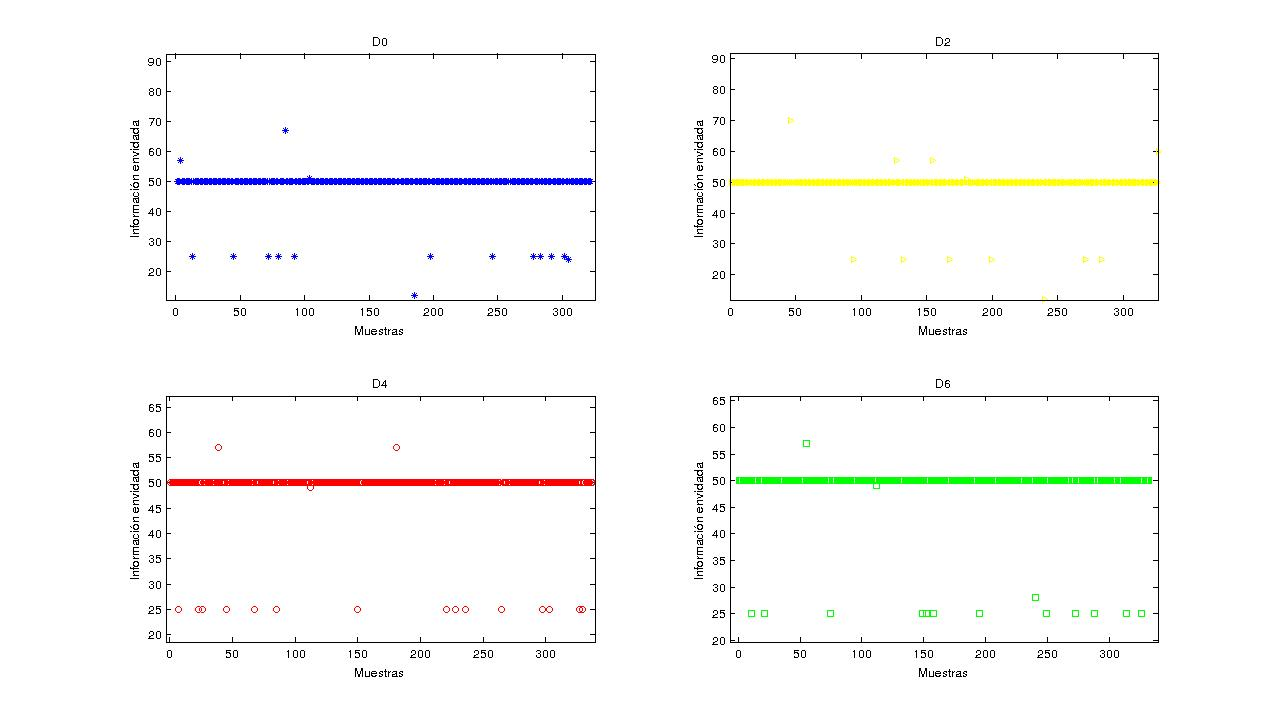
\includegraphics[width=1\textwidth]{./pics_sniffer/grafica_ejemplo.jpg}
	\caption{Prueba N$^o$ $0$}
	\label{fig:grafica_motores}
\end{figure}


Haciendo un an\'alisis similar con el resto de las pruebas detalladas en la tabla \ref{tab:pruebas} se construye la tabla \ref{tab:resumen_snif} donde se muestran los valores enviados a cada motor en promedio en todas las pruebas.\\

\begin{table}[H]
\begin{center}
\begin{tabular}{c|c|c|c|c|c|} 
\cline{2-5}
& \multicolumn{4}{c|}{\cellcolor[gray]{0.8} Valor promedio} \\ \hline
\multicolumn{1}{|c|}{\cellcolor[gray]{0.8} Prueba} & \cellcolor[gray]{0.8} D0 & \cellcolor[gray]{0.8} D2 & \cellcolor[gray]{0.8} D4 & \cellcolor[gray]{0.8} D6 & \cellcolor[gray]{0.8} Movimiento \\ \hline
\multicolumn{1}{|c|}{\cellcolor[gray]{0.8}0} & 50 & 50 & 50 & 50 & Idle \\ \hline
\multicolumn{1}{|c|}{\cellcolor[gray]{0.8}1} & 80 & 140 & 180 & 140 & $a_z=cte\neq 0$\\ \hline
\multicolumn{1}{|c|}{\cellcolor[gray]{0.8}2} & 180 & 220 & 250 & 240 & $a_z=cte\neq 0$ \\ \hline \hline
\multicolumn{1}{|c|}{\cellcolor[gray]{0.8}3} & 160 & 70 & 60 & 250 & giro seg\'un eje $z$ \\ \hline
\multicolumn{1}{|c|}{\cellcolor[gray]{0.8}4} & 50 & 200 & 200 & 100 & giro seg\'un eje $-z$\\ \hline \hline
\multicolumn{1}{|c|}{\cellcolor[gray]{0.8}5} & 250 & 160 & 140 & 50 & giro seg\'un eje $-x$\\ \hline
\multicolumn{1}{|c|}{\cellcolor[gray]{0.8}6} & 50 & 160 & 150 & 250 & giro seg\'un eje $x$ \\ \hline
\multicolumn{1}{|c|}{\cellcolor[gray]{0.8}7} & 90 & 50 & 250 & 160 & giro seg\'un eje $-y$\\ \hline
\multicolumn{1}{|c|}{\cellcolor[gray]{0.8}8} & 110 & 250 & 50 &  100 & giro seg\'un eje $y$\\ \hline
\end{tabular} 
\caption{Resumen de los resultados obtenidos}
\label{tab:resumen_snif}
\end{center}
\end{table}

En la tabla \ref{tab:resumen_snif_add} se muestran los registros a los que se mandaron datos para cada dirección.

\begin{table}[H]
\begin{center}
\begin{tabular}{c|c|c|c|c|} 
\cline{2-5}
& \cellcolor[gray]{0.8} D0 & \cellcolor[gray]{0.8} D2 & \cellcolor[gray]{0.8} D4 & \cellcolor[gray]{0.8} D6 \\ \hline
\multicolumn{1}{|c|}{\cellcolor[gray]{0.8}Registro} & A2 & A2 & A2 & A2\\ \hline
\end{tabular} 
\caption{Resumen de las direcciones obtenidas}
\label{tab:resumen_snif_add}
\end{center}
\end{table}

De las anteriores 2 tablas se pueden sacar algunas conclusiones que se analizar\'an en la secci\'on \ref{sec:conclu}.

\section{Prueba de arranque}
\label{sec:arranque}

En esta secci\'on se analiza la secuencia de arranque del cuadric\'optero. Se parte con la palanca de elevaci\'on al m\'inimo y se procede a moverla para arrancar los motores.\\

Mientras la palanca de elevaci\'on se mantiene al m\'inimo, se le env\'ia el valor 0 a los cuatro motores. Al mover la palanca, luego de un \emph{tiempo muerto} donde las l\'ineas quedan inactivas, se les empieza a enviar el valor correspondiente a cada motor, como se puede ver en la figura \ref{fig:snif_arranque_lejos}.

\begin{figure}[h!]
	\centering
	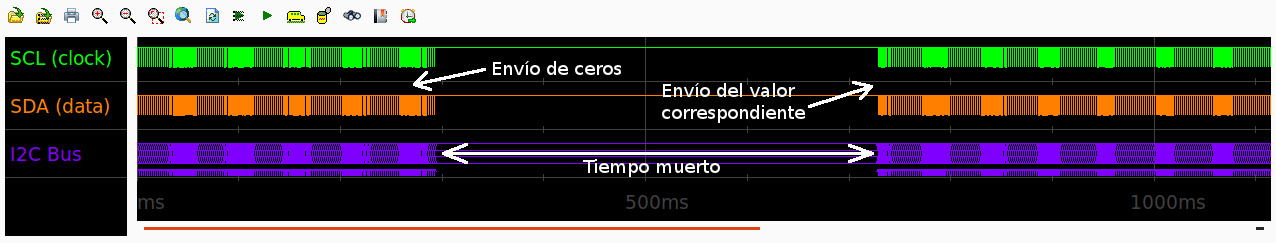
\includegraphics[width=1\textwidth]{./pics_sniffer/snif_arranque_lejos.png}
	\caption{Arranque}
	\label{fig:snif_arranque_lejos}
\end{figure}

Observando m\'as detenidamente los comandos enviados se pueden obtener algunas conclusiones importantes. En la gran mayor\'ia de los casos se env\'ian los comandos en el orden $D2\rightarrow D4\rightarrow D6\rightarrow D0$ y se guardan en el registro 0xA2 del esclavo. Pero se pueden observar dos importantes diferencias en la el \'ultimo comando que se manda a cada motor antes de arrancar, es decir, el \'ultimo comando en la tanda de ceros mostrada en la figura \ref{fig:snif_arranque_lejos}:

\begin{figure} [h!]
\centering
  \subfloat[Tanda normal de ceros]{\label{fig:snif_arranque_ceros}
  		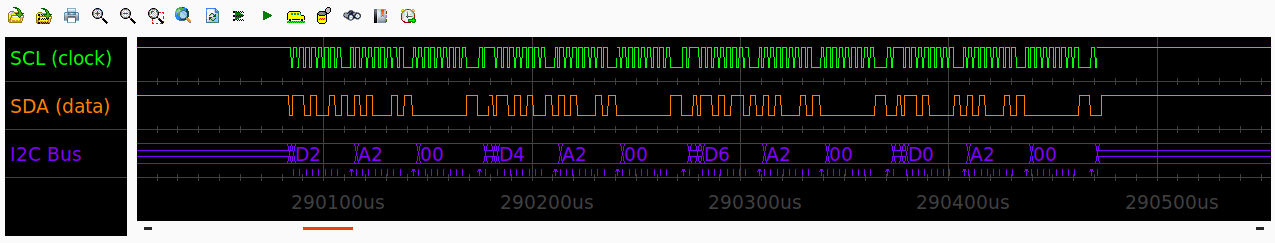
\includegraphics[width=1\textwidth]{./pics_sniffer/snif_arranque_ceros.png}} \\
  \subfloat[Última tanda de ceros]{\label{fig:snif_arranque_ultimos_ceros} 
  		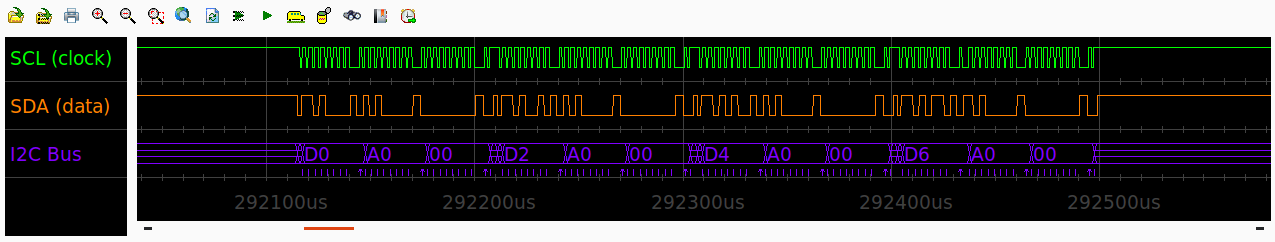
\includegraphics[width=1\textwidth]{./pics_sniffer/snif_arranque_ultimos_ceros.png}}
  \caption{Env\'io de ceros}
  \label{fig:snif_arranque_cerca}
\end{figure}

\begin{itemize}
\item \textbf{El orden en el que se env\'ian datos a los motores no es mismo} que el anterior. En este caso el orden es: $D0\rightarrow D2\rightarrow D4\rightarrow D6$.
\item \textbf{El registro en el que se escriben los datos es 0xA0}
\end{itemize}

En la figura \ref{fig:snif_arranque_ceros} se muestra una tanda regular de ceros y en la figura \ref{fig:snif_arranque_ultimos_ceros} se muestra la \'ultima tanda de ceros mencionada.\\

Dichas diferencias se pueden observar claramente al graficar todos los datos obtenidos, como se muestra en la figura \ref{fig:arranque}. Se grafica para cada motor el valor que le llega (figura \ref{fig:arranque_val}) y el registro donde el valor es escrito (figura \ref{fig:arranque_reg}). Al analizar los resultados gr\'aficamente resulta evidente el cambio en el registro al terminar de mandar los ceros. En la figura \ref{fig:arranque_val} se puede observar que el \'ultimo cero que se manda a los motores, se manda alrededor de la muestra 150. Analizando la figura \ref{fig:arranque_reg} es clar\'isimo que alrededor de la muestra 150, el registro al que se env\'ian los comandos cambia al valor 160 (0xA0), tal como se hab\'ia observado anteriormente.

\begin{figure} [h!]
\centering
  \subfloat[Valores enviados a los motores]{\label{fig:arranque_val}
  		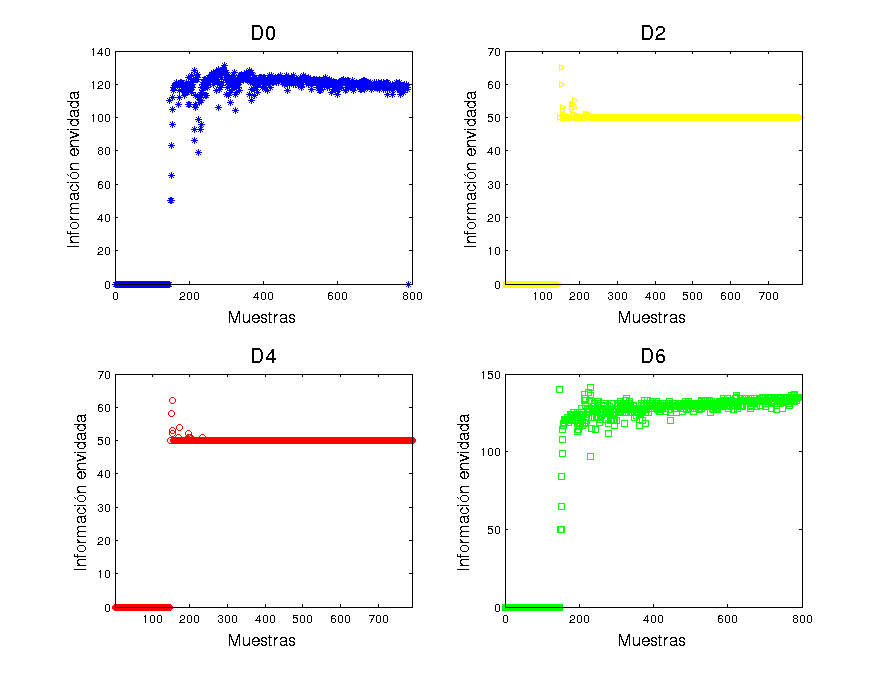
\includegraphics[width=.5\textwidth]{./pics_sniffer/arranque_val.png}}
  \subfloat[Registro al que se env\'ia el valor]{\label{fig:arranque_reg} 
  		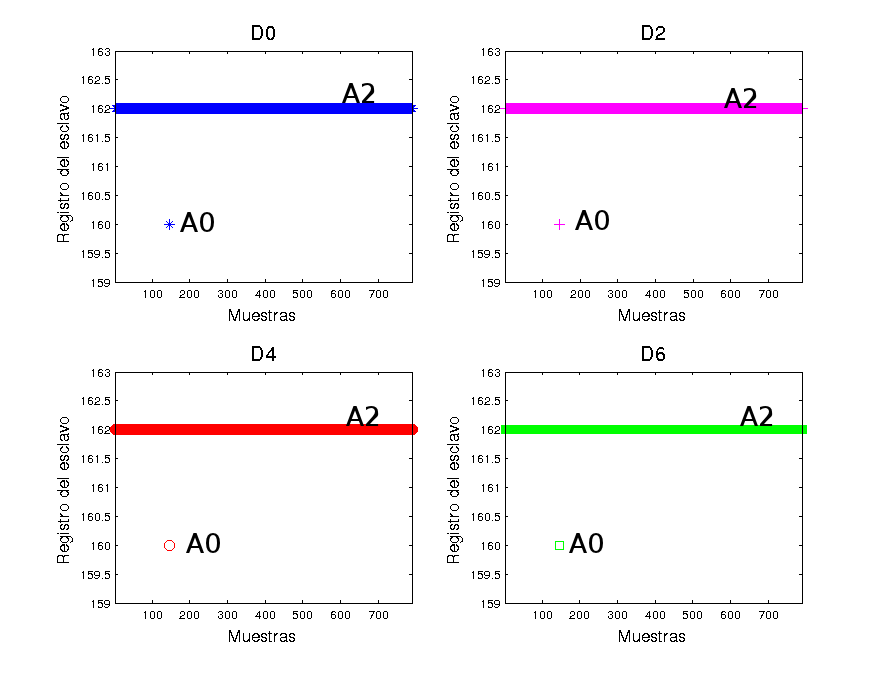
\includegraphics[width=.5\textwidth]{./pics_sniffer/arranque_reg.png}}
  \caption{Arranque}
  \label{fig:arranque}
\end{figure}


\section{Prueba de frenado}
\label{sec:frenado}
Se procede del mismo modo que en la prueba anterior (secci\'on \ref{sec:arranque}), analizando los comandos enviados a los motores a la hora de apagarlos. Se realiza una prueba an\'aloga a la anterior partiendo de los motores funcionando y bajando al m\'inimo la palanca de elevaci\'on, causando que estos se detengan.\\

Una vez que se lleva la palanca de elevaci\'on al m\'inimo, los motores se apagan y se permanece enviando ceros a los motores en el orden $D2\rightarrow D4\rightarrow D6\rightarrow D0$. Se pueden obtener algunas conclusiones importantes de la \'ultima tanda de valores distintos de cero enviados (comandos que provocan el frenado de los motores), mostrada en la figura \ref{fig:snif_frenado}:
\begin{itemize}
\item \textbf{El orden en el que se env\'ian datos es $D0\rightarrow D2\rightarrow D4\rightarrow D6$}
\item \textbf{El registro en el que se escriben los datos es 0xA1}
\end{itemize}

\begin{figure}[h!]
	\centering
	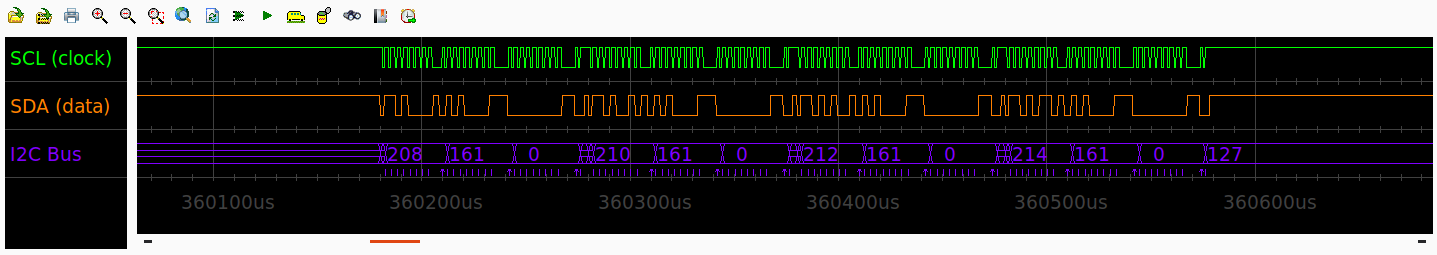
\includegraphics[width=1\textwidth]{./pics_sniffer/snif_frenado.png}
	\caption{Frenado}
	\label{fig:snif_frenado}
\end{figure}

Se presenta tambi\'en un an\'alisis gr\'afico en la figura \ref{fig:frenado}. En este caso, a diferencia del de la secci\'on \ref{sec:arranque}, no es posible divisar con claridad el registro 0xA1 (161) en la figura \ref{fig:frenado_reg}, ya que se escriben comandos a una cantidad importante de registros diferentes.\\

\begin{figure} [h!]
\centering
  \subfloat[Valores enviados a los motores]{\label{fig:frenado_val}
  		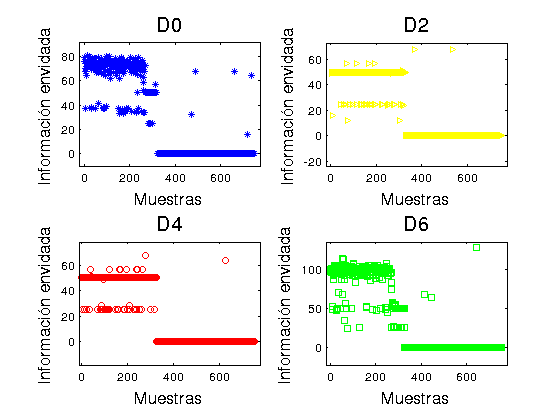
\includegraphics[width=.5\textwidth]{./pics_sniffer/frenado_val.png}}
  \subfloat[Registro al que se env\'ia el valor]{\label{fig:frenado_reg} 
  		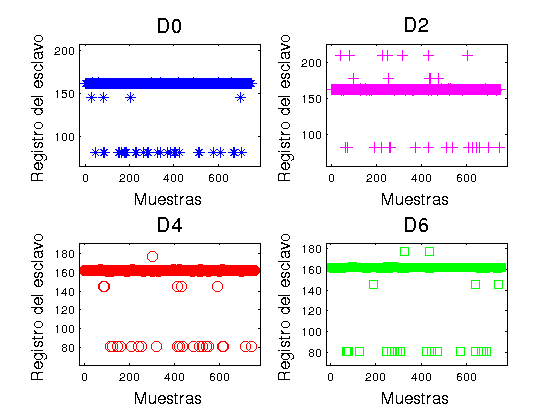
\includegraphics[width=.5\textwidth]{./pics_sniffer/frenado_reg.png}}
  \caption{Frenado}
  \label{fig:frenado}
\end{figure}

Avalados por la prueba realizada en la secci\'on \ref{sec:MSP} que se ver\'a luego, se puede afirmar que la aparici\'on de otros registros (por ejemplo los n\'umeros 81, 145, etc) son causados por el propio proceso de intervención en los buses de comunicación y no son el comando transmitido a los motores. Analicemos por ejemplo el valor 81. Es claro que el resultado de dividir el valor 162 (correspondiente al conocido registro 0xA2) entre 2 es 81, por lo cual parece probable que haya sido generado por un error del analizador lógico, ya que un corrimiento hacia la derecha de un bit en una palabra binaria es equivalente a realizar una divisi\'on entre 2. Es probable entonces que el sniffer haya incluido un bit en 0 antes de la verdadera palabra y haya descartado el \'ultimo bit, causando una aparente divisi\'on entre 2. M\'as graficamente:\\

\begin{center} 162 = 10100010 $\rightarrow$ \color{green}0\color{black}1010001\color{red}\xcancel{0}\color{black} = 81\\
\end{center}

En verde se muestra el bit agregado y en rojo el eliminado.

\section{Conclusiones}
\label{sec:conclu}

\begin{itemize}
\item La comunicaci\'on entre el amo y los esclavos por medio del protocolo $i^2c$ se lleva a cabo mediante un  formato del tipo:
\begin{quote}\textit{Direcci\'on esclavo - Lugar de memoria donde guardar dato - dato}\end{quote}
\item Dicho formato se repite para todos los esclavos
\item Cada esclavo recibe una actualizaci\'on de estado (un dato nuevo) cada $2 ms$
\item La velocidad m\'inima de funcionamiento se logra enviando el valor 50
\item La velocidad m\'axima de funcionamiento se logra enviando el valor 250
\item Cuando el mando de Elevaci\'on del control se encuentra al m\'inimo, se les env\'ia el valor 0 a los cuatro motores peri\'odicamente con el formato mencionado.
\item La direcci\'on de memoria interna de todos los esclavos donde se guardan los datos recibidos por el maestro es siempre 0x$A2$ (\'o $162$), a excepci\'on del arranque y el frenado.
\item El \'ultimo comando enviado antes de arrancar se guarda en el registro 0xA0, comando que se interpreta como una orden de arranque.
\item El \'ultimo comando enviado antes de frenar se guarda en el registro 0xA1, comando que se interpreta como una orden de frenado.
\item El orden normal en el que se env\'ian los comandos es $D2\rightarrow D4\rightarrow D6\rightarrow D0$, menos en los casos descriptos en los 2 puntos anteriores donde el orden es $D0\rightarrow D2\rightarrow D4\rightarrow D6$. Se comprobó, experimentalmente, que no es necesario alterar el orden en el que se env\'ian los comandos para lograr arrancar y frenar los motores.
\item La correspondencia entre las direcciones y los motores se muestra en la figura \ref{fig:correspondencias}. El motor con direcci\'on 0xD0 es el de adelante, el motor con direcci\'on 0xD4 es el de atr\'as y mir\'andolo de frente el de la izquierda se corresponde con 0xD0, y el de la derecha con 0xD6
\item Las direcciones 0xD0, 0xD2, 0xD4 y 0xD6 (de 8 bits) en realidad no refieren \'unicamente a direccionamiento, sino que incluyen adem\'as el bit de lectura/escritura, por lo cual cada esclavo tendr\'a una \'unica direcci\'on de 7 bits. Notar que las direcciones 0xD0 a 0xD6 al pasarlas a binario todas terminan en 0, lo cual implica que se tratan de comandos de escritura. Al omitir el \'ultimo bit se obtienen las direcciones (sin incluir el bit de lectura/escritura) como se puede ver a continuaci\'on:
\begin{eqnarray}
\mathrm{0xD0} (11010000) &\longrightarrow &\mathrm{0x68} (1101000) \\
\mathrm{0xD2} (11010010) &\longrightarrow &\mathrm{0x69} (1101001) \\
\mathrm{0xD4} (11010100) &\longrightarrow &\mathrm{0x6A} (1101010) \\
\mathrm{0xD6} (11010110) &\longrightarrow &\mathrm{0x6B} (1101011) 
\end{eqnarray}
Las direcciones de los motores son entonces: \textbf{0x68}, \textbf{0x69}, \textbf{0x6A}, \textbf{0x6B}.
\item En las pruebas 0, 1, 2, 5, 6 y 7 se observa que la suma del valor promedio enviado al motor D0 m\'as el enviado a la direcci\'on D2 es similar a la suma de los valores entregados a los motores con direcci\'on D4 y D6, lo cual implica un equilibrio en los pares realizados en ambos sentidos. 
\end{itemize}

\begin{figure}[h!]
	\centering
	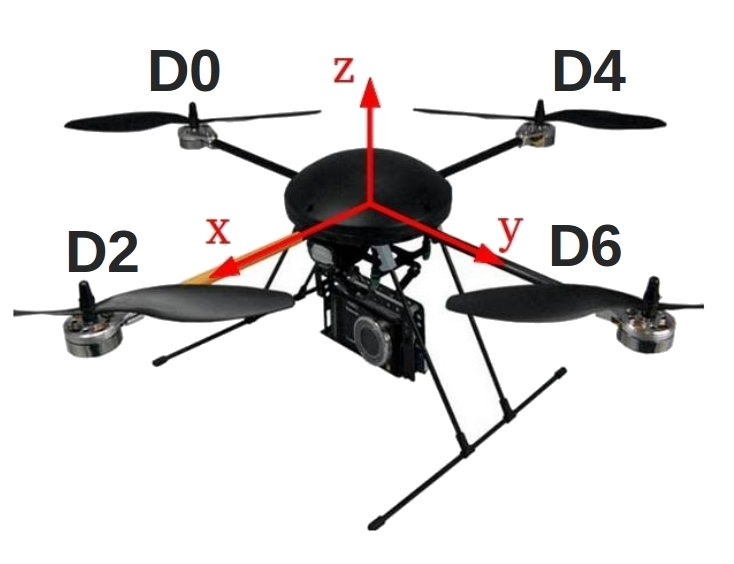
\includegraphics[width=0.4\textwidth]{./pics_sniffer/correspondencias.jpg}
	\caption{correspondencias}
	\label{fig:correspondencias}
\end{figure}

\section{Verificaciones}
Se presentan diversas verificaciones realizadas para corroborar la veracidad de las conclusiones extraídas. Adem\'as de la corroboraci\'on experimental utilizando el puerto $i^2c$ de la Beagleboard y logrando hacer funcionar los motores, previamente se realizaron 2 verificaciones adicionales:
\begin{itemize}
	\item \textbf{i2cdetect}: comando enviado desde la \emph{BeagleBoard} por el puerto \emph{i2c-2}.
	\item \textbf{MSP430F5438}: microcontrolador que se programa como esclavo con una de las direcciones de un ESC.
\end{itemize}

\subsection*{i2cdetect}
Utilizando la librer\'ia \emph{i2c Tools}\footnote{http://www.lm-sensors.org/wiki/i2cToolsDocumentation} con la Beagleboard es posible enviar el comando \textbf{i2cdetect}, el cual ``pregunta'' a todos los esclavos presentes en el bus por su direcci\'on. El resultado en terminal es el siguiente
\begin{verbatim}
root@beagleboard:~# i2cdetect -r 2
WARNING! This program can confuse your I2C bus, cause data loss and worse!
I will probe file /dev/i2c-2 using read byte commands.
I will probe address range 0x03-0x77.
Continue? [Y/n] y

     0  1  2  3  4  5  6  7  8  9  a  b  c  d  e  f
00:          -- -- -- -- -- -- -- -- -- -- -- -- -- 
10: -- -- -- -- -- -- -- -- -- -- -- -- -- -- -- -- 
20: -- -- -- -- -- -- -- -- -- -- -- -- -- -- -- -- 
30: -- -- -- -- -- -- -- -- -- -- -- -- -- -- -- -- 
40: -- -- -- -- -- -- -- -- -- -- -- -- -- -- -- -- 
50: -- -- -- -- -- -- -- -- -- -- -- -- -- -- -- -- 
60: -- -- -- -- -- -- -- -- 68 69 6a 6b -- -- -- -- 
70: -- -- -- -- -- -- -- --
\end{verbatim}

Puede verse claramente que las direcciones de los esclavos obtenidas por la funci\'on mencionada son: \textbf{0x68}, \textbf{0x69}, \textbf{0x6A}, \textbf{0x6B}.

\subsection*{MSP430F5438}
\label{sec:MSP}
\begin{wrapfigure}{r}{0.5\textwidth}
	\begin{center}
	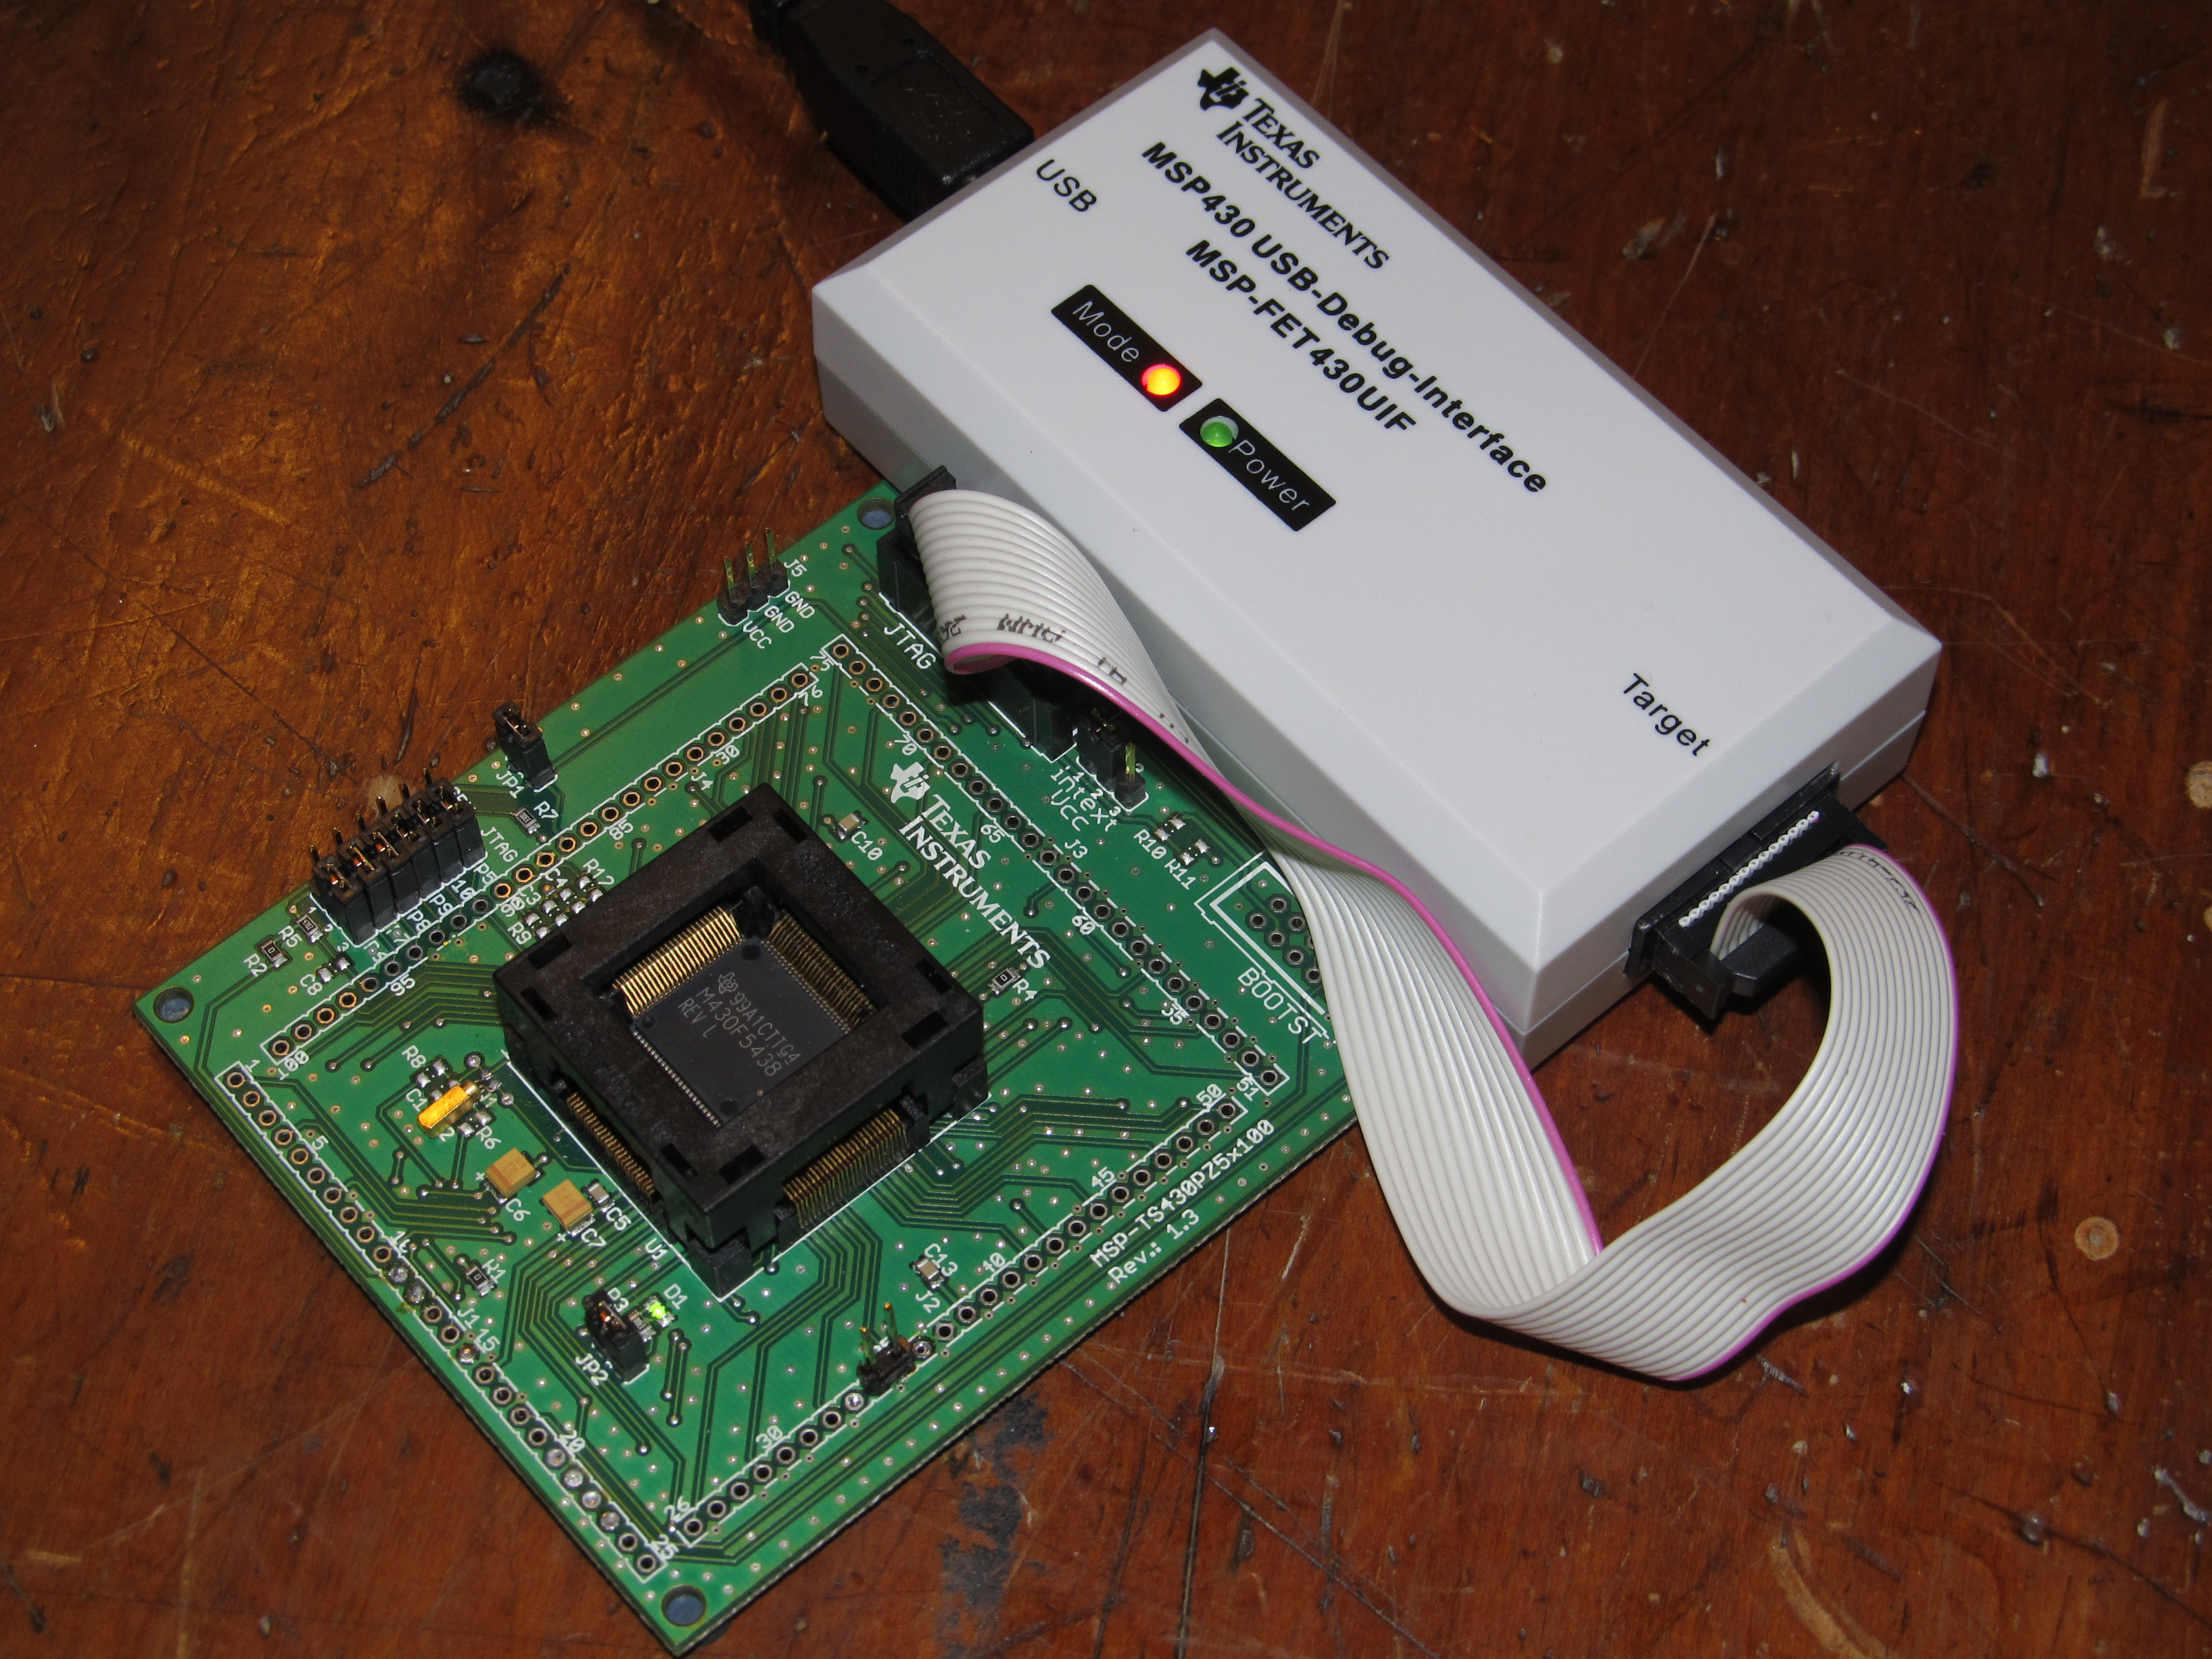
\includegraphics[width=0.4\textwidth]{./pics_sniffer/MSP430F5438.jpg}
	\end{center}
	\vspace{-20pt}
	\caption{MSP430F5438}
	\label{fig:MSP430F5438}
\end{wrapfigure}

El MSP430F5438 (ver figura \ref{fig:MSP430F5438}) posee un puerto $i^2c$ habilitado para su utilizaci\'on. Se configurara como esclavo con la direcci\'on 0x68 y se guardan en una variable los comandos recibidos en el bus. De este modo se logra independizarse de los problemas que pueda introducir el sniffer y se obtiene exactamente el comando transmitido al esclavo presente en dicha direcci\'on.\\

Luego, analizando la variable donde se guardan los comandos, es posible obtener informaci\'on m\'as concluyente. En la figura \ref{fig:MSP_arranque} se muestran los resultados obtenidos al adquirir datos en un arranque, mientras que en la figura \ref{fig:MSP_frenado} se muestran los resultados obtenidos al adquirir datos al frenar.

\begin{figure} [h!]
\centering
  \subfloat[Valores enviados a los motores]{\label{fig:MSP_arranque_val}
  		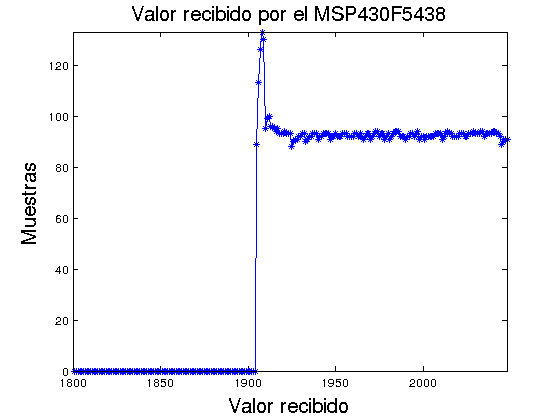
\includegraphics[width=.5\textwidth]{./pics_sniffer/MSP_arranque_val.png}}
  \subfloat[Registro al que se env\'ia el valor]{\label{fig:MSP_arranque_reg} 
  		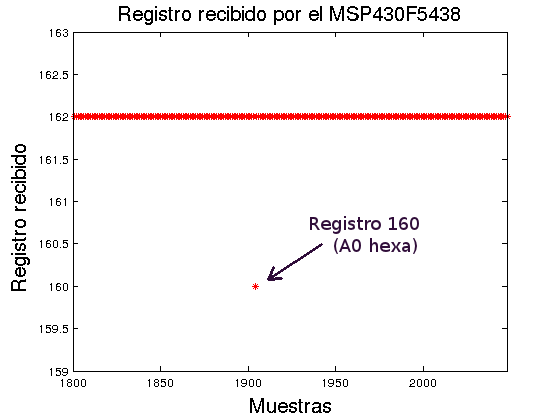
\includegraphics[width=.5\textwidth]{./pics_sniffer/MSP_arranque_reg.png}}
  \caption{Arranque detectado por el MSP430F5438}
  \label{fig:MSP_arranque}
\end{figure}


\begin{figure} [h!]
\centering
  \subfloat[Valores enviados a los motores]{\label{fig:MSP_frenado_val}
  		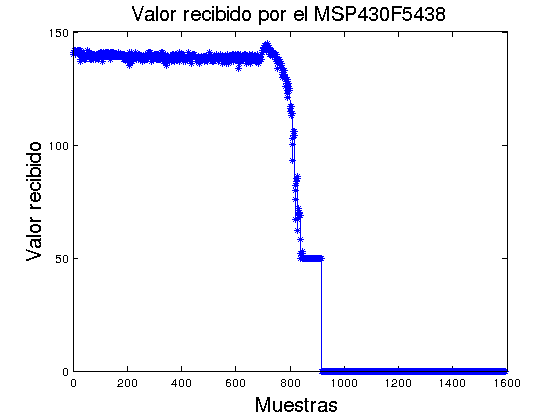
\includegraphics[width=.5\textwidth]{./pics_sniffer/MSP_frenado_val.png}}
  \subfloat[Registro al que se env\'ia el valor]{\label{fig:MSP_frenado_reg} 
  		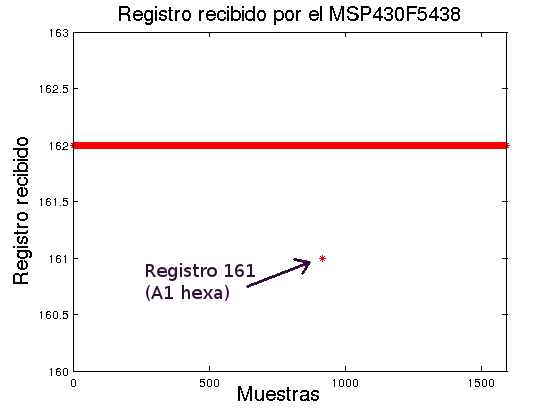
\includegraphics[width=.5\textwidth]{./pics_sniffer/MSP_frenado_reg.png}}
  \caption{Frenado}
  \label{fig:MSP_frenado}
\end{figure}

Estas \'ultimas dos figuras son las corroboraciones m\'as concluyentes que se obtuvieron. Ratifica y deja bien en claro lo antes dicho sobre los registros: \textbf{para el arranque se escribe en la direcci\'on 0xA0 del esclavo y para el frenado se escribe en la direcci\'on 0xA1.}\\

A su vez sirve de confirmaci\'on para los errores del sniffeado detectados en la secci\'on \ref{sec:frenado}.

\end{document}